\subsection{Simulation}

The behaviour of the impementation was tested by writing small programs that would try to provoke certain errors and write debug data to the registers.
They programs were written in a simplified assembly variant and then passed through the assembler to produce signals constants which could be pasted directly into tb\_toplevel.vhd.
The simulation was then run, and the resulting data in the registers was compared to the desired data corresponding to the assembly.

Alu operations, memory operations, forwarding, jumping, branching and flushing were all tested and proved to work correctly. The test programs can be found in the appendix, and there are currently no known bugs.

\subsection{Timing Simulation}

\begin{figure}[ht]
    \centering
    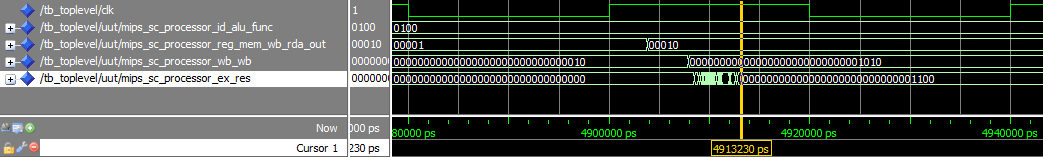
\includegraphics[scale=0.5]{figures/TimingSimulation.png}
    \caption{Timing diagram for critical path} 
    \label{fig:timing}
\end{figure}

Figure \ref{fig:timing} is a timing diagram showing the output from the ALU, which is the end of the critical path that starts at the ex/mem pipeline register and goes through the bottom link mux, the forwarding unit, the forwarding mux, and into the ALU.
The time from a rising clock edge to a the output is stable is shown to be $13.230$ ns, which translates to a maximum clock speed of about $75$ Mhz.
This is very close to the max clock speed of $77.442$ MHz reported by the synthesis tool.

\subsection{Verification}

By following the extensive procedure in the compendium \cite[p.47]{lab-compendium} and using the supplied user\_logic.vhd and main.c files, the design was added to the MicroBlaze framework and compiled to a bit file, before uploading it to an AvNet Development Board by using AvProg.


\begin{figure}[ht]
    \centering
    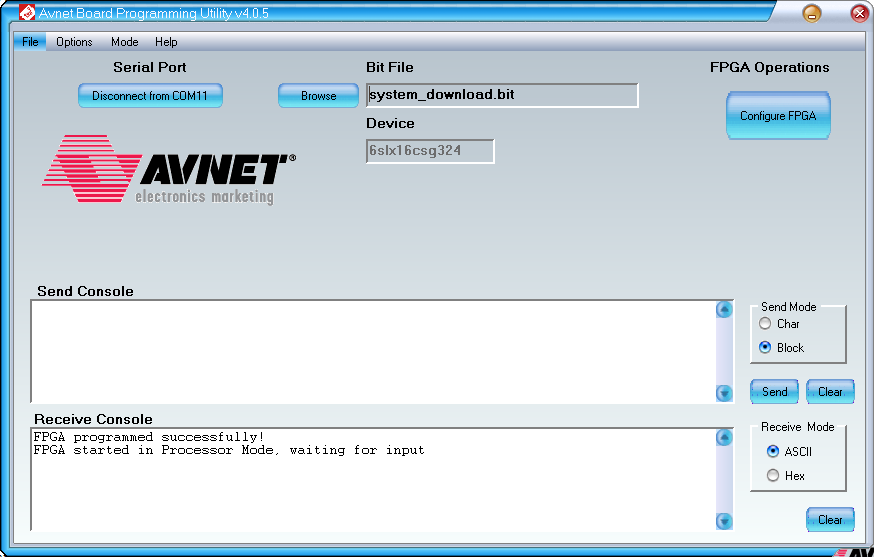
\includegraphics[scale=0.5]{figures/AVNET.png}
    \caption{FPGA programmed successfully} 
    \label{fig:avprog}
\end{figure}

\todo{stuff}

